\documentclass[]{article}
\usepackage{lmodern}
\usepackage{amssymb,amsmath}
\usepackage{ifxetex,ifluatex}
\usepackage{fixltx2e} % provides \textsubscript
\ifnum 0\ifxetex 1\fi\ifluatex 1\fi=0 % if pdftex
  \usepackage[T1]{fontenc}
  \usepackage[utf8]{inputenc}
\else % if luatex or xelatex
  \ifxetex
    \usepackage{mathspec}
  \else
    \usepackage{fontspec}
  \fi
  \defaultfontfeatures{Ligatures=TeX,Scale=MatchLowercase}
\fi
% use upquote if available, for straight quotes in verbatim environments
\IfFileExists{upquote.sty}{\usepackage{upquote}}{}
% use microtype if available
\IfFileExists{microtype.sty}{%
\usepackage{microtype}
\UseMicrotypeSet[protrusion]{basicmath} % disable protrusion for tt fonts
}{}
\usepackage[margin=1in]{geometry}
\usepackage{hyperref}
\hypersetup{unicode=true,
            pdftitle={visit Simulation Report},
            pdfauthor={visit package},
            pdfborder={0 0 0},
            breaklinks=true}
\urlstyle{same}  % don't use monospace font for urls
\usepackage{longtable,booktabs}
\usepackage{graphicx,grffile}
\makeatletter
\def\maxwidth{\ifdim\Gin@nat@width>\linewidth\linewidth\else\Gin@nat@width\fi}
\def\maxheight{\ifdim\Gin@nat@height>\textheight\textheight\else\Gin@nat@height\fi}
\makeatother
% Scale images if necessary, so that they will not overflow the page
% margins by default, and it is still possible to overwrite the defaults
% using explicit options in \includegraphics[width, height, ...]{}
\setkeys{Gin}{width=\maxwidth,height=\maxheight,keepaspectratio}
\IfFileExists{parskip.sty}{%
\usepackage{parskip}
}{% else
\setlength{\parindent}{0pt}
\setlength{\parskip}{6pt plus 2pt minus 1pt}
}
\setlength{\emergencystretch}{3em}  % prevent overfull lines
\providecommand{\tightlist}{%
  \setlength{\itemsep}{0pt}\setlength{\parskip}{0pt}}
\setcounter{secnumdepth}{0}
% Redefines (sub)paragraphs to behave more like sections
\ifx\paragraph\undefined\else
\let\oldparagraph\paragraph
\renewcommand{\paragraph}[1]{\oldparagraph{#1}\mbox{}}
\fi
\ifx\subparagraph\undefined\else
\let\oldsubparagraph\subparagraph
\renewcommand{\subparagraph}[1]{\oldsubparagraph{#1}\mbox{}}
\fi

%%% Use protect on footnotes to avoid problems with footnotes in titles
\let\rmarkdownfootnote\footnote%
\def\footnote{\protect\rmarkdownfootnote}

%%% Change title format to be more compact
\usepackage{titling}

% Create subtitle command for use in maketitle
\providecommand{\subtitle}[1]{
  \posttitle{
    \begin{center}\large#1\end{center}
    }
}

\setlength{\droptitle}{-2em}

  \title{visit Simulation Report}
    \pretitle{\vspace{\droptitle}\centering\huge}
  \posttitle{\par}
    \author{visit package}
    \preauthor{\centering\large\emph}
  \postauthor{\par}
      \predate{\centering\large\emph}
  \postdate{\par}
    \date{2019-08-15}


\begin{document}
\maketitle

{
\setcounter{tocdepth}{3}
\tableofcontents
}
\clearpage

\hypertarget{simulation-parameters}{%
\section{Simulation Parameters}\label{simulation-parameters}}

\begin{longtable}[]{@{}ll@{}}
\toprule
Variables & Values\tabularnewline
\midrule
\endhead
Number of doses & 3\tabularnewline
decision cuts & 0.65, 0.65, 0.65\tabularnewline
etas & 0.1, 0.3\tabularnewline
probability model & NONPARA\tabularnewline
cohort size & 5\tabularnewline
level size & 10\tabularnewline
n rep & 100\tabularnewline
n core & 3\tabularnewline
\bottomrule
\end{longtable}

\clearpage

\hypertarget{trueps-plots}{%
\section{Trueps Plots}\label{trueps-plots}}

\hypertarget{trueps-plots-1}{%
\subsection{Trueps Plots 1}\label{trueps-plots-1}}

Probability of DLT risk and immune response:\\
\includegraphics{report_files/figure-latex/TRUEPS1-1.pdf}

\clearpage

\hypertarget{trueps-plots-2}{%
\subsection{Trueps Plots 2}\label{trueps-plots-2}}

Probability of each scenario:\\
\includegraphics{report_files/figure-latex/TRUEPS2-1.pdf}

\clearpage

\hypertarget{simulation-results}{%
\section{Simulation Results}\label{simulation-results}}

\begin{table}[ht]
\centering
\begin{tabular}{rrrr}
  \hline
 & 1 & 2 & 3 \\ 
  \hline
Frequency & 54.00 & 15.00 & 11.00 \\ 
  \% & 54.00 & 15.00 & 11.00 \\ 
   \hline
\end{tabular}
\end{table}
\begin{table}[ht]
\centering
\begin{tabular}{rrrr}
  \hline
 & stage 1 & stage 2 & total \\ 
  \hline
level 1 & 5.00 & 4.00 & 9.00 \\ 
  level 2 & 4.00 & 1.75 & 5.75 \\ 
  level 3 & 1.30 & 0.80 & 2.10 \\ 
   \hline
\end{tabular}
\end{table}
\begin{table}[ht]
\centering
\begin{tabular}{rrrrrrr}
  \hline
 & No T, No R & No T, R & T, No R & T,R & T & R \\ 
  \hline
level 1 stage 1 & 3.26 & 0.85 & 0.74 & 0.15 & 0.89 & 1.00 \\ 
  level 1 stage 2 & 2.59 & 0.68 & 0.60 & 0.13 & 0.73 & 0.81 \\ 
  level 1 total & 5.85 & 1.53 & 1.34 & 0.28 & 1.62 & 1.81 \\ 
  level 2 stage 1 & 2.55 & 0.55 & 0.76 & 0.14 & 0.90 & 0.69 \\ 
  level 2 stage 2 & 1.08 & 0.31 & 0.24 & 0.12 & 0.36 & 0.43 \\ 
  level 2 total & 3.63 & 0.86 & 1.00 & 0.26 & 1.26 & 1.12 \\ 
  level 3 stage 1 & 0.77 & 0.31 & 0.15 & 0.07 & 0.22 & 0.38 \\ 
  level 3 stage 2 & 0.49 & 0.12 & 0.17 & 0.02 & 0.19 & 0.14 \\ 
  level 3 total & 1.26 & 0.43 & 0.32 & 0.09 & 0.41 & 0.52 \\ 
   \hline
\end{tabular}
\end{table}
\begin{table}[ht]
\centering
\begin{tabular}{rrrrrr}
  \hline
 & N & Toxic & Ineffective & Safe,Effective & Effective,Safety concern \\ 
  \hline
level 1 stage 1 & 100.00 & 20.00 & 0.00 & 0.00 & 80.00 \\ 
  level 1 stage 2 & 80.00 & 0.00 & 0.00 & 11.25 & 88.75 \\ 
  level 2 stage 1 & 80.00 & 33.75 & 22.50 & 0.00 & 43.75 \\ 
  level 2 stage 2 & 35.00 & 5.71 & 20.00 & 5.71 & 68.57 \\ 
  level 3 stage 1 & 26.00 & 26.92 & 11.54 & 0.00 & 61.54 \\ 
  level 3 stage 2 & 16.00 & 0.00 & 31.25 & 12.50 & 56.25 \\ 
   \hline
\end{tabular}
\end{table}
\begin{table}[ht]
\centering
\begin{tabular}{rrrrr}
  \hline
 & Toxic & Ineffective & Safe,Effective & Effective,Safety concern \\ 
  \hline
level 1 stage 1 & 0.39 & 0.00 & 0.22 & 0.40 \\ 
  level 1 stage 2 & 0.23 & 0.00 & 0.24 & 0.54 \\ 
  level 2 stage 1 & 0.46 & 0.29 & 0.07 & 0.18 \\ 
  level 2 stage 2 & 0.26 & 0.29 & 0.13 & 0.32 \\ 
  level 3 stage 1 & 0.38 & 0.25 & 0.15 & 0.22 \\ 
  level 3 stage 2 & 0.23 & 0.33 & 0.13 & 0.30 \\ 
   \hline
\end{tabular}
\end{table}
\begin{table}[ht]
\centering
\begin{tabular}{rrrr}
  \hline
 & Mean & LB & UB \\ 
  \hline
level 1 stage 1 & 0.27 & 0.14 & 0.57 \\ 
  level 1 stage 2 & 0.21 & 0.08 & 0.33 \\ 
  level 2 stage 1 & 0.30 & 0.14 & 0.57 \\ 
  level 2 stage 2 & 0.22 & 0.08 & 0.42 \\ 
  level 3 stage 1 & 0.26 & 0.14 & 0.43 \\ 
  level 3 stage 2 & 0.21 & 0.08 & 0.33 \\ 
   \hline
\end{tabular}
\end{table}
\begin{table}[ht]
\centering
\begin{tabular}{rrrr}
  \hline
 & Mean & LB & UB \\ 
  \hline
level 1 stage 1 & 0.29 & 0.14 & 0.57 \\ 
  level 1 stage 2 & 0.25 & 0.08 & 0.50 \\ 
  level 2 stage 1 & 0.27 & 0.14 & 0.57 \\ 
  level 2 stage 2 & 0.28 & 0.08 & 0.51 \\ 
  level 3 stage 1 & 0.35 & 0.14 & 0.57 \\ 
  level 3 stage 2 & 0.31 & 0.16 & 0.50 \\ 
   \hline
\end{tabular}
\end{table}

\clearpage

\hypertarget{observation}{%
\section{Observation}\label{observation}}

vtTrack Plots\\
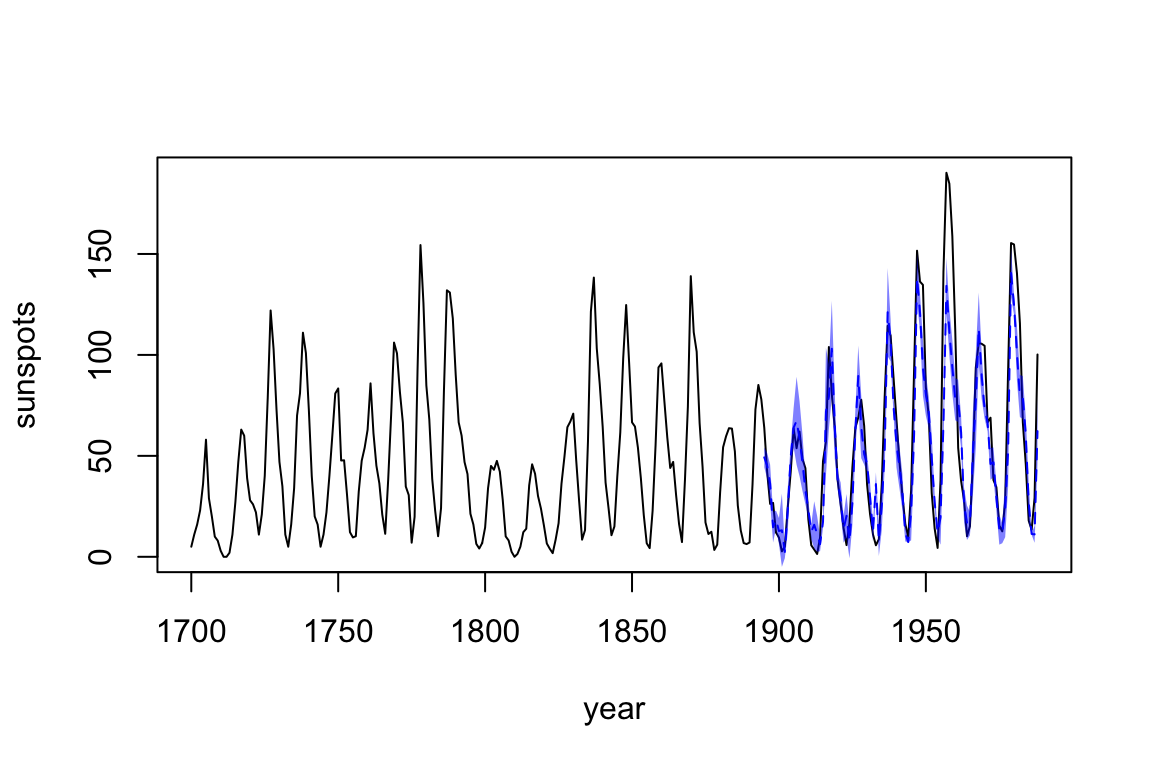
\includegraphics{report_files/figure-latex/unnamed-chunk-3-1.pdf}

\begin{table}[ht]
\centering
\begin{tabular}{rrrrr}
  \hline
1 & 2 & 3 & 4 & 5 \\ 
  \hline
1 & 0 & 0 & 0 & 0 \\ 
  2 & 0 & 0 & 0 & 0 \\ 
  3 & 0 & 0 & 0 & 0 \\ 
   \hline
\end{tabular}
\end{table}

\clearpage

\hypertarget{observation-interim}{%
\section{Observation Interim}\label{observation-interim}}

\begin{verbatim}
## 
## Level 1
\end{verbatim}

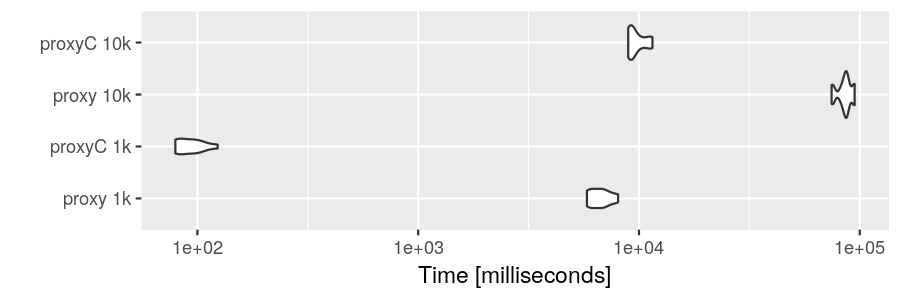
\includegraphics{report_files/figure-latex/unnamed-chunk-4-1.pdf}

\begin{verbatim}
## 
## Level 2
\end{verbatim}

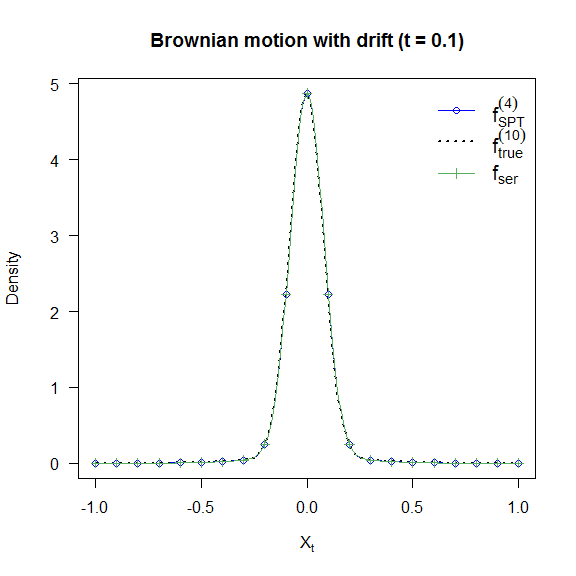
\includegraphics{report_files/figure-latex/unnamed-chunk-4-2.pdf}

\begin{verbatim}
## 
## Level 3
\end{verbatim}

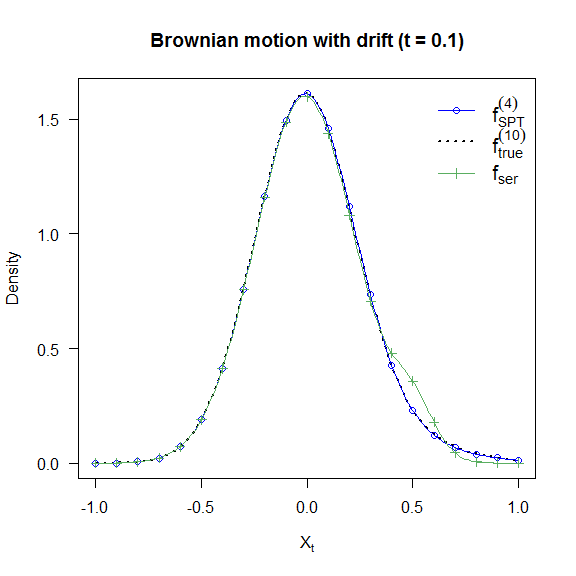
\includegraphics{report_files/figure-latex/unnamed-chunk-4-3.pdf}


\end{document}
